\documentclass[tikz,border=10pt]{standalone}
\usetikzlibrary{calc}

\begin{document}
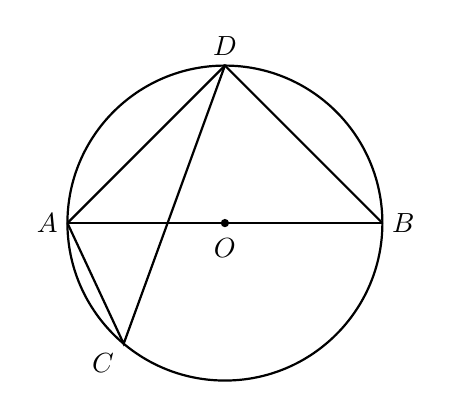
\begin{tikzpicture}
    % --- 参数定义 ---
    \def\r{2} % 设置圆的半径
    
    % --- 坐标点定义 ---
    \coordinate (O) at (0,0);
    \coordinate (A) at (-\r,0);
    \coordinate (B) at (\r,0);
    % 使用极坐标放置 D 和 C，可根据需要调整角度
    \coordinate (D) at (90:\r); 
    \coordinate (C) at (230:\r);
    
    % --- 绘制图形 ---
    % 绘制圆
    \draw[thick] (O) circle (\r);
    
    % 绘制直径及其它线段
    \draw[thick] (A) -- (B);    % 直径 AB
    \draw[thick] (A) -- (D) -- (B); % 上半部分三角形
    \draw[thick] (A) -- (C) -- (D); % 连接 AC 和 CD
    
    % --- 标记点 ---
    \fill (O) circle (1.5pt) node[below=2pt] {$O$};
    \node[left] at (A) {$A$};
    \node[right] at (B) {$B$};
    \node[above] at (D) {$D$};
    \node[below left] at (C) {$C$};
    
\end{tikzpicture}
\end{document}